\section{Model and Methodology}

Investigating the physics of of a thermoacoustic interaction requires the resolving of the full non-linear acoustics in the combustion system -- this might typically be a plenum, inlet, combustor and exhaust -- as well as the highly local reaction and diffusion phenomena located at the flame. In the case of a deflagration in a tube, the acoustics span the whole tube and a premixed flame and surrounding hydrodynamics will be located in one relatively small region of this tube. It would be natural, then, to fully resolve the flame and hydrodynamics by a fully simulated region and leave the which are the dominant effect upstream and downstream of the flame to be modelled separately. Assume at the simulation inflow that we can decompose the pressure and velocity fields as $u = \overline{u} + u'$ and $p = \overline{p} + p'$, where $\overline{\cdot}$ represents the average field at the inflow and $\cdot'$ represents fluctuations with zero mean. Then the value of $\overline{u} \pm c$ determines the speed of acoustic waves through the tube. Under a linear assumption for these acoustics -- i.e. the assumption that $ρ = \overline{ρ}$ such that $ρ' = 0$ or equivalently that acoustics do not interact with each other -- then the convection of an acoustic wave in a headwind and tailwind will cancel out. This results in a representative time delay $τ$ for the acoustic wave to leave the simulation domain, travel a distance $l$ both ways up- or downstream, and reenter:
\begin{equation}
τ = \frac{l}{c + u} + \frac{l}{c - u} = \frac{2l}{c} \, \frac{1}{1 - \Ma} \approx \frac{2l}{c}
\end{equation}
since under the deflagration approximation $\Ma \ll 1$. This is the time delay we will associate with the simulation inflow and outflow to represent their length scale via the delayed reentry of these acoustic into the inflow and outflow after a delay $τ_{\rm{U}}$ and $τ_{\rm{D}}$ respectively. This solves the linear acoustic problem in the tube upstream and downstream of the flame to leading order in Mach number. We refer to this non-DNS domain by the acoustic or fictitious domain or region.

% Add arrow for DNS velocity
% use τ
\begin{figure}[t]
\centering
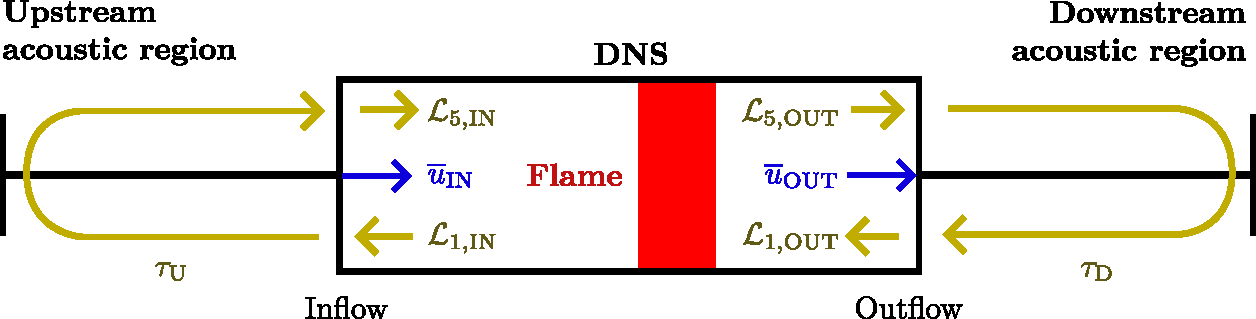
\includegraphics[scale=0.65]{assets/imgs/delay_bc_model.pdf}
\caption{Simple diagram for the simulation model.}
\label{fig:delay-model}
\end{figure}

To fit this model into the existing characteristic boundary formulation provided by NSCBC and LODI, we assume that we can store all of the outgoing acoustics as $\cl{L}_{\text{outgoing acoustic}}(t, \vb{y})$ where $\cl{L}_{\text{outgoing acoustic}}$ is the continuous outgoing field and the vector $\vb{y}$ parameterises the given connected inflow or outflow (this is a scalar value $y$ for 2 dimensional problems with vertical inflow or outflow). For a rectangular two-dimensional horizontal tube, this becomes $\cl{L}_{1/5}(t, y)$ where the outgoing acoustic is $\cl{L}_{1}$ for left-side boundaries and $\cl{L}_{5}$ for right-side boundaries (inflows and outflows respectively in this report). A simple diagram of the acoustic behaviour is shown in \fig{fig:delay-model} as acoustic values leave and reenter the DNS domain repeatedly. Continuing with this two-dimensional example, we would impose the delayed acoustic reentry by imposing at the left-side inflow that $\cl{L}_{5}(t, y) = \cl{L}_{5, \rm{nonreflect}}(t, y) + \cl{L}_{1}(t - τ, y)$ where the first term $\cl{L}_{5, \rm{nonreflect}}$ is the required condition described in the previous chapter to stop the outgoing acoustic from being immediately reflected. Under this model, we are implicitly assuming each location at the boundary has its own one-dimensional acoustic approximation being made. For the rest of the report we instead use a simpler formulation which averages the acoustics across the boundary as they leave:
\begin{subequations}
\begin{equation}
\cl{L}_{5}(t, y) = \cl{L}_{5, nonreflect}(t, y) + \langle \cl{L}_{1}(t - τ_{\rm{U}}, \cdot) \rangle_{\rm{IN}}
\end{equation}
for inflows and
\begin{equation}
\cl{L}_{1}(t, y) = \cl{L}_{1, nonreflect}(t, y) + \langle \cl{L}_{5}(t - τ_{\rm{D}}, \cdot) \rangle_{\rm{OUT}}
\end{equation}
\end{subequations}
%(NOT SURE WHAT TO DO IF THESE WAVES DO NOT FULLY REFLECT?)
for outflows, where $\langle\,\cdot\,\rangle_{\rm{IN/OUT}}$ represents averaging over inflow or outflow boundary values respectively. This corresponds to a single one-dimensional approximation being made for each boundary, which is of course only valid for thin-enough computational domains. We refer to these boundary conditions as \emph{Acoustic Delay Characteristic Boundary Conditions} (ADCBC). Since we are modelling the reaction Navier-Stokes equations, we must also impose that all other incoming $\cl{L}$ values vanish at the inflow so that no entropy, shear or mass waves enter the domain. Note that now no relaxation terms are used on either boundary -- this marks the main difference between ADCBC and NSCBC. Relaxation terms are traditionally used under the NSCBC formulation to ensure the dependent variables -- inflow velocities $\vb{u}=(u, v)$, temperature or density and mass fractions and especially outflow pressure -- do not drift as characteristic waves leave the domain, not to return under perfectly non-reflecting conditions. Given that the acoustic waves will be returning under ADCBC, we do not need these relaxation terms for inflow normal velocity ($u$ in our vertical boundaries) or outflow pressure as they are closed by the full reflection of these acoustic waves. Note that if relaxation terms were imposed on top of the delayed reflections, we would be applying a further well-posing condition to a problem which is already well-posed. For the other variables, relaxation terms may be kept, but we have chosen to remove them under the assumption that the simulation is strongly one-dimensional and inert at the boundary. That is, no significant shear, entropy or mass waves should be leaving these boundaries, so the related dependent variables $v$, $T$, $Y_α$ will not drift. All that is left is to apply the diffusive BCs as the remaining physical BCs. Nothing here changes with \cite{sutherland2003ImprovedBoundaryConditions}, where they use the zero normal flux conditions \equ{eqn:znf}. A further consideration to make is what happens when the acoustic field is strong enough that $\abs{\overline{u}} < \abs{u'}$ at the inflow or outflow. Usually we expect this to happen at the inflow first since $\abs{\overline{u}_{\rm{IN}}} > \abs{\overline{u}_{\rm{OUT}}}$, i.e. the acoustic field has become large enough that the inflow has become an outflow. 


% - inflows may switch to outflows. To account for this, we simply check if the boundary is has u.n > 0 for inflow and otherwise is outflow and apply the corresponding conditions for L and diffusive conditions

% - Later on, this definition of $\cl{L}_{5}(t, y)$ can be extended to include a forcing term if that is desirable e.g. to simulate secondary thermoacoustic instability response
%Later on, these definitions for $\cl{L}_{1/5}$ can be extended to include an imposed acoustic field ifi that is desirable, e.g. to simulate a secondary thermoacoustic instability response. 
% - Technically this method could also be extended to arbitrary numbers of delay boundaries with any boundary normal, but this is not explored in this work (or likely future work)



\section{Implementation}

% - Brief summary: To outline the method again, we will be introducing a delay into the acoustics to model an extended acoustic domain which is not part of the DNS region by using non-reflecting characteristic boundaries and storing the acoustics which leave the domain. These acoustics are then simply reintroduced after the relevant time delay.

% Now discretise the above formulation
% - The sunset code uses, like all other numerical techniques, a discretised temporal domain to integrate forward in time.
% - Hence, we already only have the outgoing characteristic L values at discrete times and cannot recover $\cl{L}_{1}(t - τ, y')$ when $t - τ$ does not lie on a time step. Furthermore, the step size taken by a typical combustion simulation is likely to oversample the acoustic field at the boundary, resulting in a much higher memory footprint than is required. This, along with the variable time steps the SUNSET uses means that it is reasonable to use a sample rate for $\cl{L}_{1}(t_sample, y)$ values which is higher than the maximum time step size used. Call this time step size $δt_{\rm{sample}}$ which is the sample period we aim for with ADCBC.
% - In reality the time steps will be of varying sizes due to the variable time steps, refer to the sample time as $\{t_s\}_{s=0}^{N_{\rm{samp}}}$ and the sampled characteristics as $\{\cl{L}_{1, s}\}_{s=0}^{N_{\rm{samp}}}$ where $s\in\bb{Z}$ enumerates these sample times and $t_{N_{\rm{samp}}}$ is the most recent sample time.
% - define $\{\cl{L}_{1, s}\}_{s=0}^{N_{\rm{samp}}}$ values from < >_ ..
% - In order to evaluate $\cl{L}_{1}(t - τ)$ then, we simply interpolate between these $\cl{L}_{1}$ values at $t' = t - τ$.



\subsection{Code Schematic}

% We now outline the ADCBC method as it is implemented into the sunset code.
% - Because the time delay is only a finite length, clearly the oldest sample value we should need is $\cl{L}_{1}(t', y')$ where $t' \approx t - τ - δt_{\rm{sample}}$. Hence we only need to store the finite number of samples $\cl{T} = \{t_s\}_{s=0}^{N_{\rm{samp}}} \cup [t - τ - δt_{\rm{sample}}, t]$ at any given time. For as long as τ remains bounded, the size of $\cl{T}$ remains bounded.
% - this means as long as we know the maximum delay time $τ$ occurring in a given simulation (usually τ values will be constant ... not explained moving boundaries yet????) we can always store t_s, L_s in a contiguous portion of memory which the delay boundaries are allocated at the beginning of the simulation.
% - We do this using a one-sided queue data structure, which is coded as a wrapper around a contiguous array using a FIFO system. t and L values sampled at the present time can be added to the end of their respective queues, and values which are required for interpolation are found at the beginning of the queue. Once they are no longer needed for an accurate interpolation of L_1, they are 'popped' (AKA removed) from the queue
% - If a special data structure is not used for these samples, then the data would continuously slink through memory in a way where \emph{contiguity} cannot be enforced
% - Note that a linked list could also be used here although these are much more complex to implement, and far slower to traverse for interpolation values. Also, the main benefit of a linked list is the O(1) deletion of random samples, which we do not require here.

\begin{figure}[t]
\centering
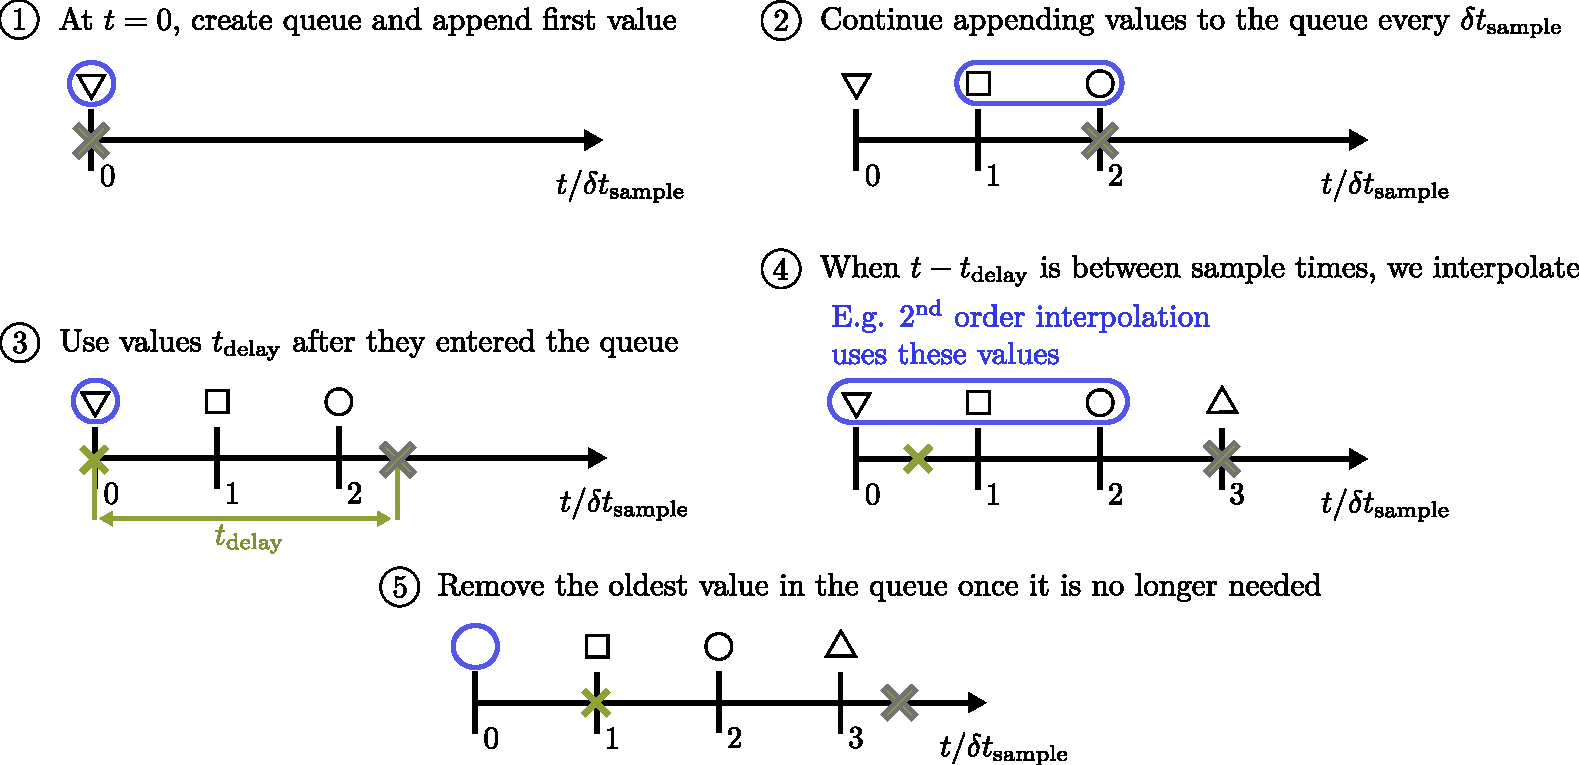
\includegraphics[scale=0.65]{assets/imgs/delay_bc_queue.pdf}
\label{fig:delay-queue}
\caption{HOW THE BOUNDARY SAMPLING AND DELAY WORK. WHAT DO SHAPES REPRESENT?? GREY CROSS IS CURRENT SIMULATION TIME, GOLD CROSS IS THAT TIME MINUS THE TIME DELAY. CHANGING TIME DELAY IS NOT SHOWN HERE.}
\end{figure}

% - The queue system used is illustrated in \fig{fig:delay-queue} in a continuous time integration for simplicity so sample times are consistent. Different shapes are used to represent the different L_1 values. The values relevant to the current step is circled in blue. The first two steps show values being appended to the queue at the beginning of the simulation until the time delay is reached in the third step. The fourth step shows which values are used for interpolation in an example second order interpolant. The fifth and final step shows old values being removed from the start of the queue 

% - on top of this, the time delay can change provided it doesn't exceed the sound speed (so multiple L values are not entering the domain at any one sample time). Time delays can be updated at each sample time assuming it doesn't change fast (actually it should change every substep???)
% - \fig{fig:schematic} illustrates the full schematic for a time integrator with two substeps per time step and uniform time step size. Sampling is performed in the (A) routine which is called every sample time preceded by a change to delay time, if required. These are circled and labelled (1) and (2) corresponding to the steps in \fig{fig:delay-queue}. Only after the full time delay $τ$ do the values from the beginning of the queue start to get used. This is shown in the labels (3) and (4) corresponding to those steps in \fig{fig:delay-queue}. Finally, step (5) removes the oldest value from the queue only once they are not needed.
% - Appending and removal from the queue happen before the queue values are used for interpolation to ensure the correct values are available in the queue for interpolation.
% - Note that the routine (U) happens every substep using as many values from the beginning of the queue as are required. The shape shown for this routine in steps (3) and (4) are just the earliest sample taken which would be used.


\begin{figure}[t]
\centering
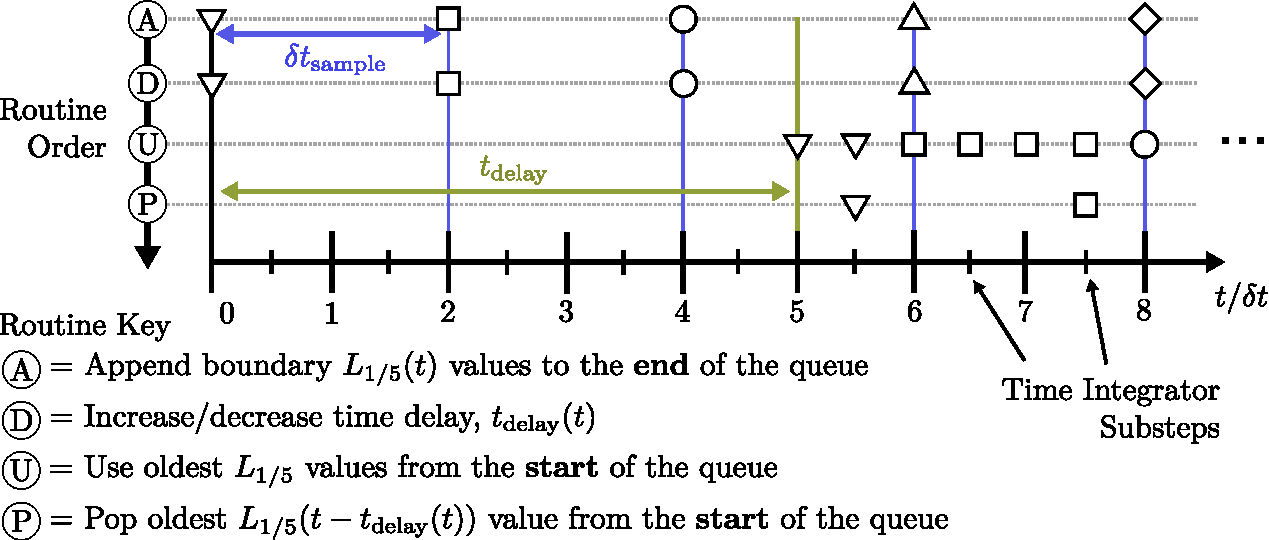
\includegraphics[scale=0.65]{assets/imgs/delay_bc_code_schematic.pdf}
\label{fig:schematic}
% A sample period $δt_{\rm{sample}} = 2δt$ is used in this example. The evaluation of routines (or procedures) are shown in order from top to bottom (starting with (D) and ending with (U), key given in the figure), left to right (beginning at $t = 0$ and showing up to $t = 8 δt$). Routines which are performed are signified by the presence of a shape representing again a different sample time. The time delay is shown in gold. 
\caption{Schematic for delay BCs implemented into a multistage time integrator. ASSUMES CONSTANT TIME STEPS. TOP TO BOTTOM, LEFT TO RIGHT. BLUE SHOWS SAMPLE TIMES, GOLD SHOWS TIME DELAY}
\end{figure}



\subsection{Sampling Error}

\begin{figure}[t]
\centering
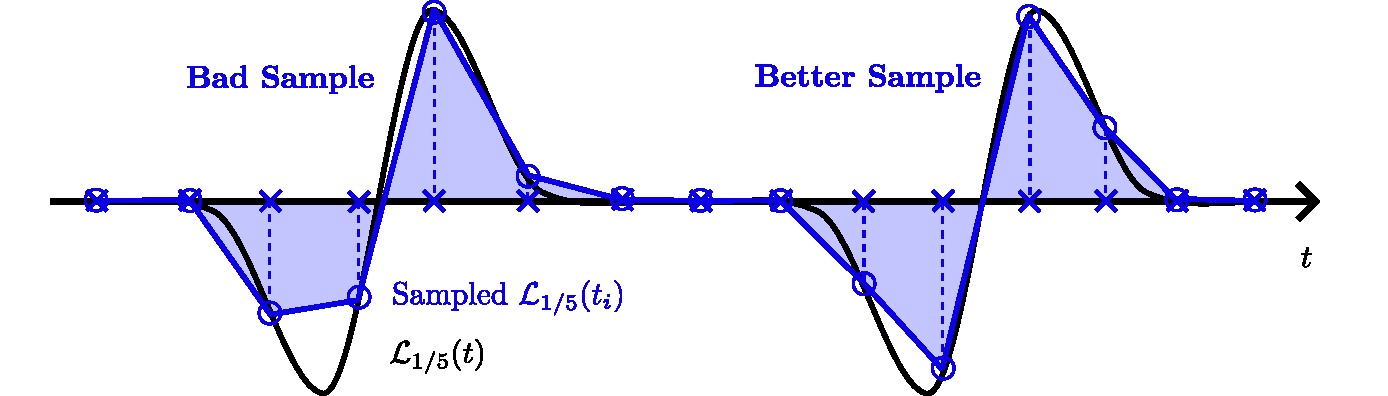
\includegraphics[scale=0.65]{assets/imgs/wave-sampling-comparison.pdf}
\caption{SAMPLING}
\label{fig:wave-sampling}
\end{figure}


% Now is a good time to bring up the sampling error
% - \fig{fig:wave-sampling} shows a representative analytic L_{1/5} field for two acoustic bumps (which is roughly the derivative of the Gaussian). Despite the same linear interpolation and sample period being used, the sampled $L$ values on the left are much worse than on the right. The same could be true for any number of samples at a constant interpolation order and sample period, where the change in phase of the sampling with the wave will always cause some inaccuracy in the integrated acoustic field. This inaccuracy results in a change to the shape of the Gaussian, e.g. a skew to one side, which feeds back into this issue such that the waves eventually fully break down
% - For the acoustic bump in this small domain this seems to happen relatively quickly because the associated acoustic frequencies of this system are higher. But, if the bump remains the same size and the tube is made longer, less bounces happen and the sampling error grows slower
% - Furthermore, there is the added effect that natural wavenumbers of these longer tubes will be lower, meaning that individual waves can be sampled better. This leads to an asymptotic behaviour of O(l^2) for values of error productions which are small (DO SOME MATHS?).



\subsection{Memory Footprint}

% - One potential disadvantage of the method is the size of queues required for the ADCBCs to hold the acoustic data since this should be available only to the processors relevant to the boundary nodes so the memory burden should be held only by those processors
% - If the memory requirement is too large (e.g. over ~4 GB), the simulations will likely crash and high-memory compute nodes will be required, which should be avoided
% - Let us now perform a simple calculation to estimate the memory required by a given acoustic delay characteristic boundary
% - Look at a single boundary under the strongly one-dimensional flow approximation. For a 1d .. (in notebook)

% - IMPORTANT POINT: regardless of how you do the calculation, the memory footprint must be significantly lower for the ADCBC formulation than it would be if the full non-linear acoustics were being solved given that only a 1D approximation is being made, the 'effective acoustic discretisation length' is much larger for ADCBC than for any simulation since the waves travel linearly and especially because we are making the strongly one-dimensional flow approximation in this report (which will be relaxed in further work).







\section{Discussion and Comparison with D-TDIBC}
% Maybe this should be in discussion chapter??


% From lit review:
%% "Since the model constants are calculated as a preprocessing step, the envelope of the acoustic response in the frequency domain may essentially be changed arbitrarily, presenting a benefit in case different pass bands are desired. Besides the inevitable drawbacks stemming from: the low-order model's inaccuracy and the requirement of a strongly one-dimensional flow at the boundary to match this model, other drawbacks remain prevalent. For one, no method to visualise acoustics residing in the fictitious, truncated domain is provided, potentially leading to a \emph{black-box} where acoustics are not immediately known. For another, the preprocessing steps are required for each value of $τ$ used. So, if the time delay were to change dynamically during the simulation (e.g. due to an expanding computational domain to ensure the flame remains within), this preprocessing may happen each step, becoming computationally costly."

% - We provide a way to visualise truncated acoustics, which they do not
% - We can add on other boundary treatments simply by including further terms into the specification of L, they instead include different boundary treatments by change the impedance envelope for different frequencies. An acoustic envelope which decays for high frequencies is actually a requirement for D-TDIBC. This has the added benefit that the ADCBC formalism can be added into existing codes already using the NSCBC formalism, under some extra requirements. The ADCBC method propose currently offers no way of modelling upstream or downstream boundary impedance effects. This also means the effectiveness of the method is dependent on the quality of the baseline nonreflecting condition
% - Both methods have very cheap boundary cost, but a pre-processing cost must be paid for D-TDIBC for a given time-delay and envelope. The time delay could change theoretically, although this is not explored in their paper.
% - They have a much lower memory footprint, since no memory of previous steps is required. We have at least two queues for each ADCBC. This could be simply extended to using a queue for each boundary node. As mentioned above, the overall memory footprint of the method should be dominated by interior nodes, especially for three-dimensional simulations
% - In both cases a strongly one-dimensional flow is required at the boundary and only the delay effects under low-amplitude acoustics are modelled




